%% \documentclass[officiallayout]{tktla}
%% \usepackage[utf8]{inputenc}
%% \usepackage{pdfpages}
%% % This package sets the margin width 
%% % (change "right" if you want them wider, but then change the 34.8pt in \note bigger too)
%% \usepackage[top=1.2in, bottom=1.5in, left=1in, right=1.6cm]{geometry}
%% \def \dvWHITE{white}
%% \def \dvBLACK{black}
%% \def \dvBLUE{blue}
%% \def \dvGREEN{green}
%% %%.72 = marker width§
%% %% 138,6: height 
%% % Use this if you have 5 articles
%% %\def \dvheight{138.6pt}
%% % Use this if you have 6 articles
%% \def \dvheight{115.5pt}
%% % Creates black box with the text given as first parameter in white
%% \newcommand\note[3] {\marginpar{\vspace{#2}\colorbox{#3}{\parbox[c][\dvheight][t]{34.8pt}{\vspace{0.3cm}\color{white}\centering\Huge{\textbf{#1}}}}}}

%% % This overlays a white box to make black box narrower, but it's not needed anymore with geometry package changing margin width
%% %\newcommand\notee[2]{\marginpar{\vspace{#1}\colorbox{#2}{               \parbox[c][\dvheight][t]{11.8pt}{              \color{white}\centering\Huge{\textbf{$\ $}}}}}}

%% \pagestyle{empty}
%% \begin{document}


\newgeometry{top=1.2in, bottom=1.5in, left=1in, right=1.6cm}

% ******************************************************************************
\chapter*{Paper I}\thispagestyle{plain}
\addcontentsline{toc}{section}{High-resolution sweep metagenomics using fast probabilistic inference}

\note{I}{-222pt}{black}
%\notee{-222pt}{\dvWHITE}

% Here it's not necessary to draw the following boxes to position right,
% and drawing them occasionally creates unwanted gray lines

%\note{II}{-100pt}{\dvWHITE}
%\notee{-126.5pt}{\dvWHITE}

%\note{III}{-5pt}{\dvWHITE}
%\notee{-126.5pt}{\dvWHITE}

%\note{IV}{-5pt}{\dvWHITE}
%\notee{-126.5pt}{\dvWHITE}

%\note{V}{-5pt}{\dvWHITE}
%\notee{-126.5pt}{\dvWHITE}

%\note{VI}{-5pt}{\dvWHITE}
%\notee{-126.5pt}{\dvWHITE}

\vspace{80pt}
% The names of the authors
\underline{Tommi Mäklin}, Teemu Kallonen, Sophia David, Christine J
Boinett, Ben Pascoe, Guillaume Méric, David M Aanensen, Edward J Feil,
Stephen Baker, Julian Parkhill, Samuel K Sheppard, Jukka Corander, and
Antti Honkela.

\vspace{10pt}
% Title of the 1st paper
\noindent\textbf{High-resolution sweep metagenomics using fast probabilistic inference}

\vspace{10pt}
% Bibliographical information of the paper, for example, of a conference paper
\noindent In
\emph{Wellcome Open Research},
\\vol. 5 issue 14, 2021.
\\doi: \href{https://doi.org/10.12688/wellcomeopenres.15639.2}{10.12688/wellcomeopenres.15639.2}.

\vspace{60pt}
% Copyright information, if the publisher is, for example, ACM
\noindent Copyright \textcopyright\ 2021 Mäklin T et al. This is an
open access article distributed under the terms of the Creative
Commons Attribution License, which permits unrestricted use,
distribution, and reproduction in any medium, provided the original
work is properly cited.

\cleardoublepage
% Including the original publication
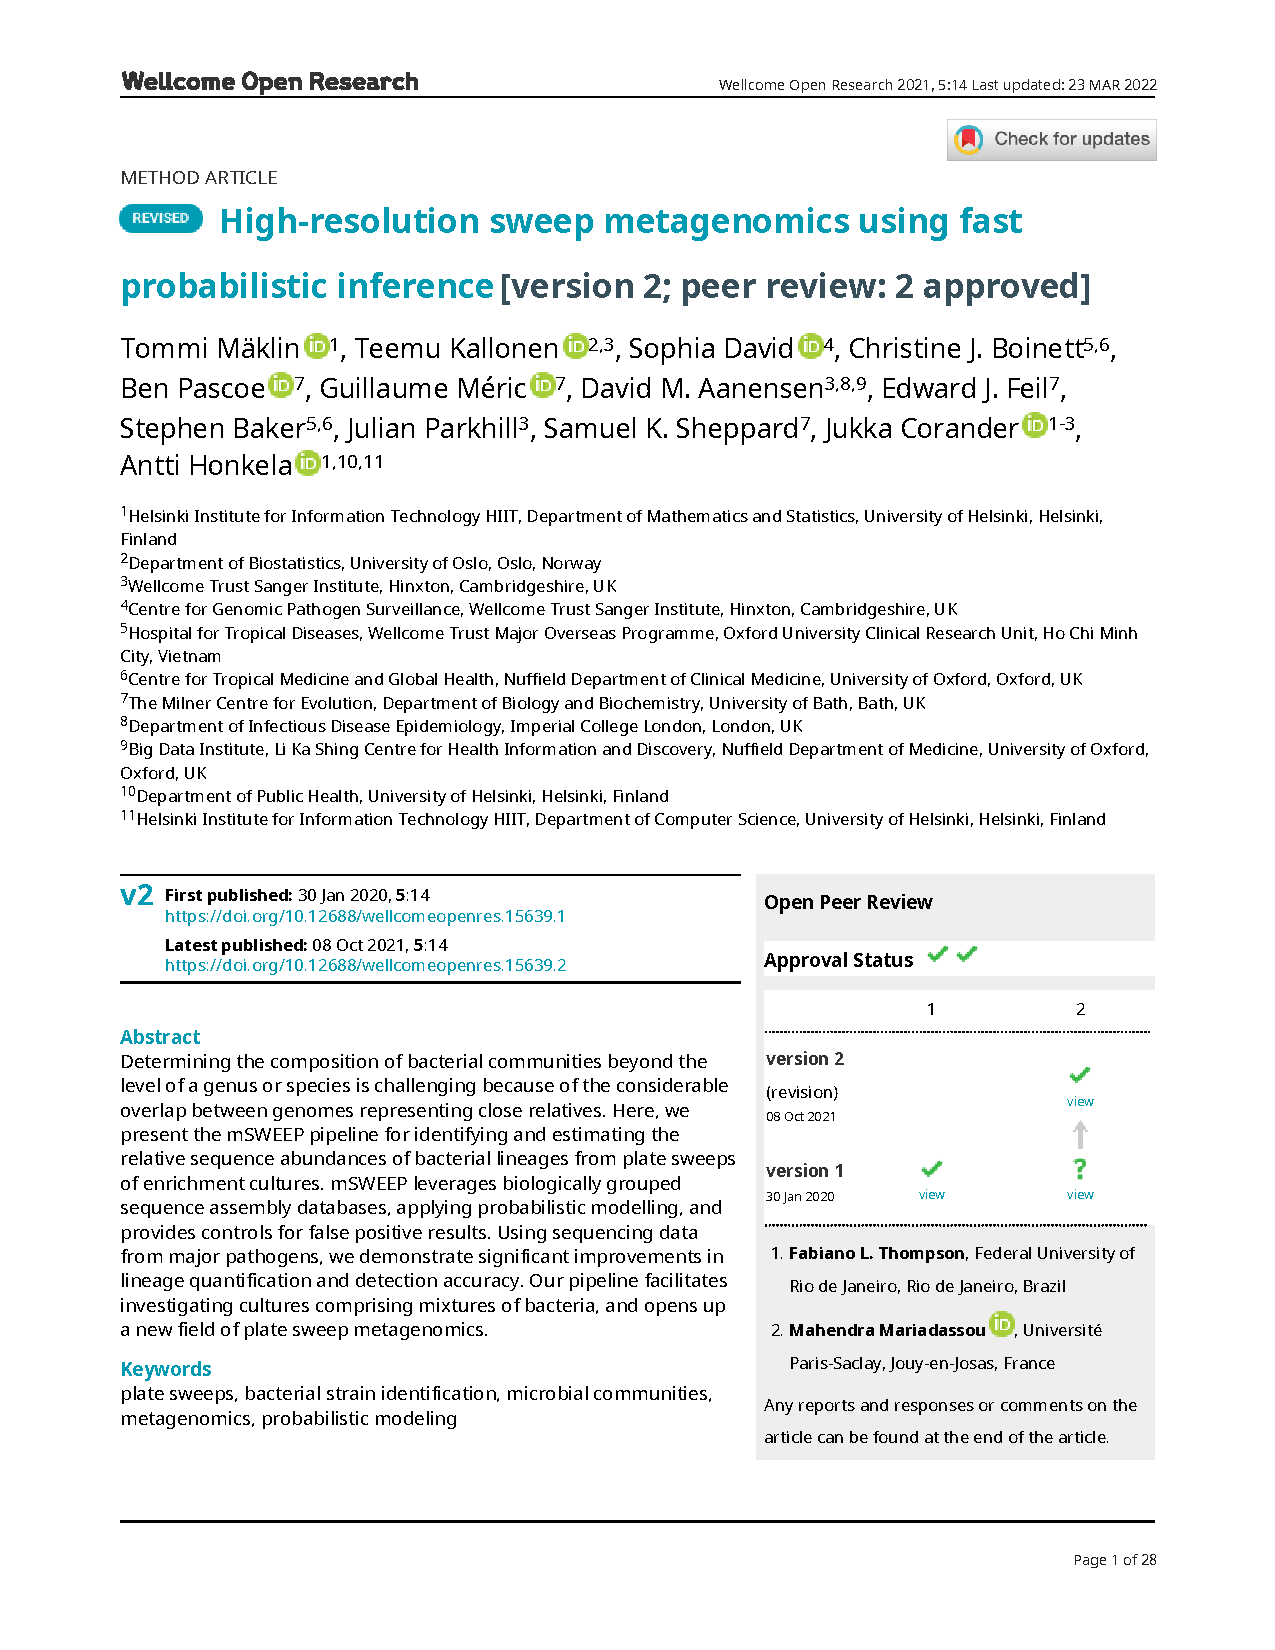
\includepdf[pages=-]{papers/maklin_high-resolution_2021.pdf}


% ******************************************************************************


\chapter*{Paper II}\thispagestyle{plain}
\addcontentsline{toc}{section}{Bacterial genomic epidemiology with mixed samples}

\note{I}{-222pt}{\dvWHITE}
%\notee{-222pt}{\dvWHITE}

\note{II}{-5pt}{black}
%\notee{-126.5pt}{\dvWHITE}

\note{III}{0pt}{\dvWHITE}
%\notee{-126.5pt}{\dvWHITE}

%% \note{IV}{-5pt}{\dvWHITE}
%% %\notee{-126.5pt}{\dvWHITE}

%% \note{V}{-5pt}{\dvWHITE}
%% %\notee{-126.5pt}{\dvWHITE}

%% \note{VI}{-5pt}{\dvWHITE}
%% %\notee{-126.5pt}{\dvWHITE}

\vspace{80pt}

% Here are the names of the authors
\underline{Tommi Mäklin}, Teemu Kallonen, Jarno Alanko, Ørjan
Samuelsen, Kristin Hegstad, Veli Mäkinen, Jukka Corander, Eva Heinz,
and Antti Honkela.

\vspace{10pt}
% Title of the 2nd paper
\noindent\textbf{Bacterial genomic epidemiology with mixed samples}

\vspace{10pt}
% Bibliographical information of the paper, for example, of a conference paper
\noindent In 
\emph{Microbial Genomics}, 
\\vol. 7 issue 11, 2021.
\\doi: \href{https://doi.org/10.1099/mgen.0.000691}{10.1099/mgen.0.000691}.

\vspace{60pt}
% Copyright information, for example, if the publisher is Springer
\noindent Copyright \textcopyright\ The Authors. This is an
open-access article distributed under the terms of the Creative
Commons Attribution License. This article was made open access via a
Publish and Read agreement between the Microbiology Society and the
corresponding author’s institution.

\cleardoublepage
% Including the original publication
\includepdf[pages=-]{papers/maklin_bacterial_2021.pdf}

% ******************************************************************************


\chapter*{Paper III}\thispagestyle{plain}
\addcontentsline{toc}{section}{Strong pathogen competition in neonatal gut colonization}

\note{I}{-222pt}{\dvWHITE}
%\notee{-222pt}{\dvWHITE}

\note{II}{-5pt}{\dvWHITE}
%\notee{-126.5pt}{\dvWHITE}

\note{III}{0pt}{black}
%\notee{-126.5pt}{\dvWHITE}

%% \note{IV}{-5pt}{\dvWHITE}
%% %\notee{-126.5pt}{\dvWHITE}

%% \note{V}{-5pt}{\dvWHITE}
%% %\notee{-126.5pt}{\dvWHITE}

%% \note{VI}{-5pt}{\dvWHITE}
%% %\notee{-126.5pt}{\dvWHITE}

\vspace{80pt}
% Here are the names of the authors
\underline{Tommi Mäklin}, Harry A Thorpe, Anna K Pöntinen, Rebecca
A Gladstone, Yan Shao, Maiju Pesonen, Alan McNally, Pål J Johnsen,
Ørjan Samuelsen, Trevor D Lawley, Antti Honkela, and Jukka
Corander.

\vspace{10pt}
% Title of the 3rd paper
\noindent\textbf{Strong pathogen competition in neonatal gut colonisation}

\vspace{10pt}
% Bibliographical information of the paper, for example, a submitted paper
\noindent Submitted, preprint available from \textit{bioRxiv}.
\\doi: \href{https://doi.org/10.1101/2022.06.19.496579}{10.1101/2022.06.19.496579}.

\vspace{60pt}
%Copyright information, when the authors have the copyright of the paper
\noindent
The copyright holder for this preprint is the author/funder, who has
granted bioRxiv a license to display the preprint in perpetuity. It is
made available under a \href{http://creativecommons.org/licenses/by/4.0/}{CC-BY 4.0 International license}.

\cleardoublepage
% Including the original publication
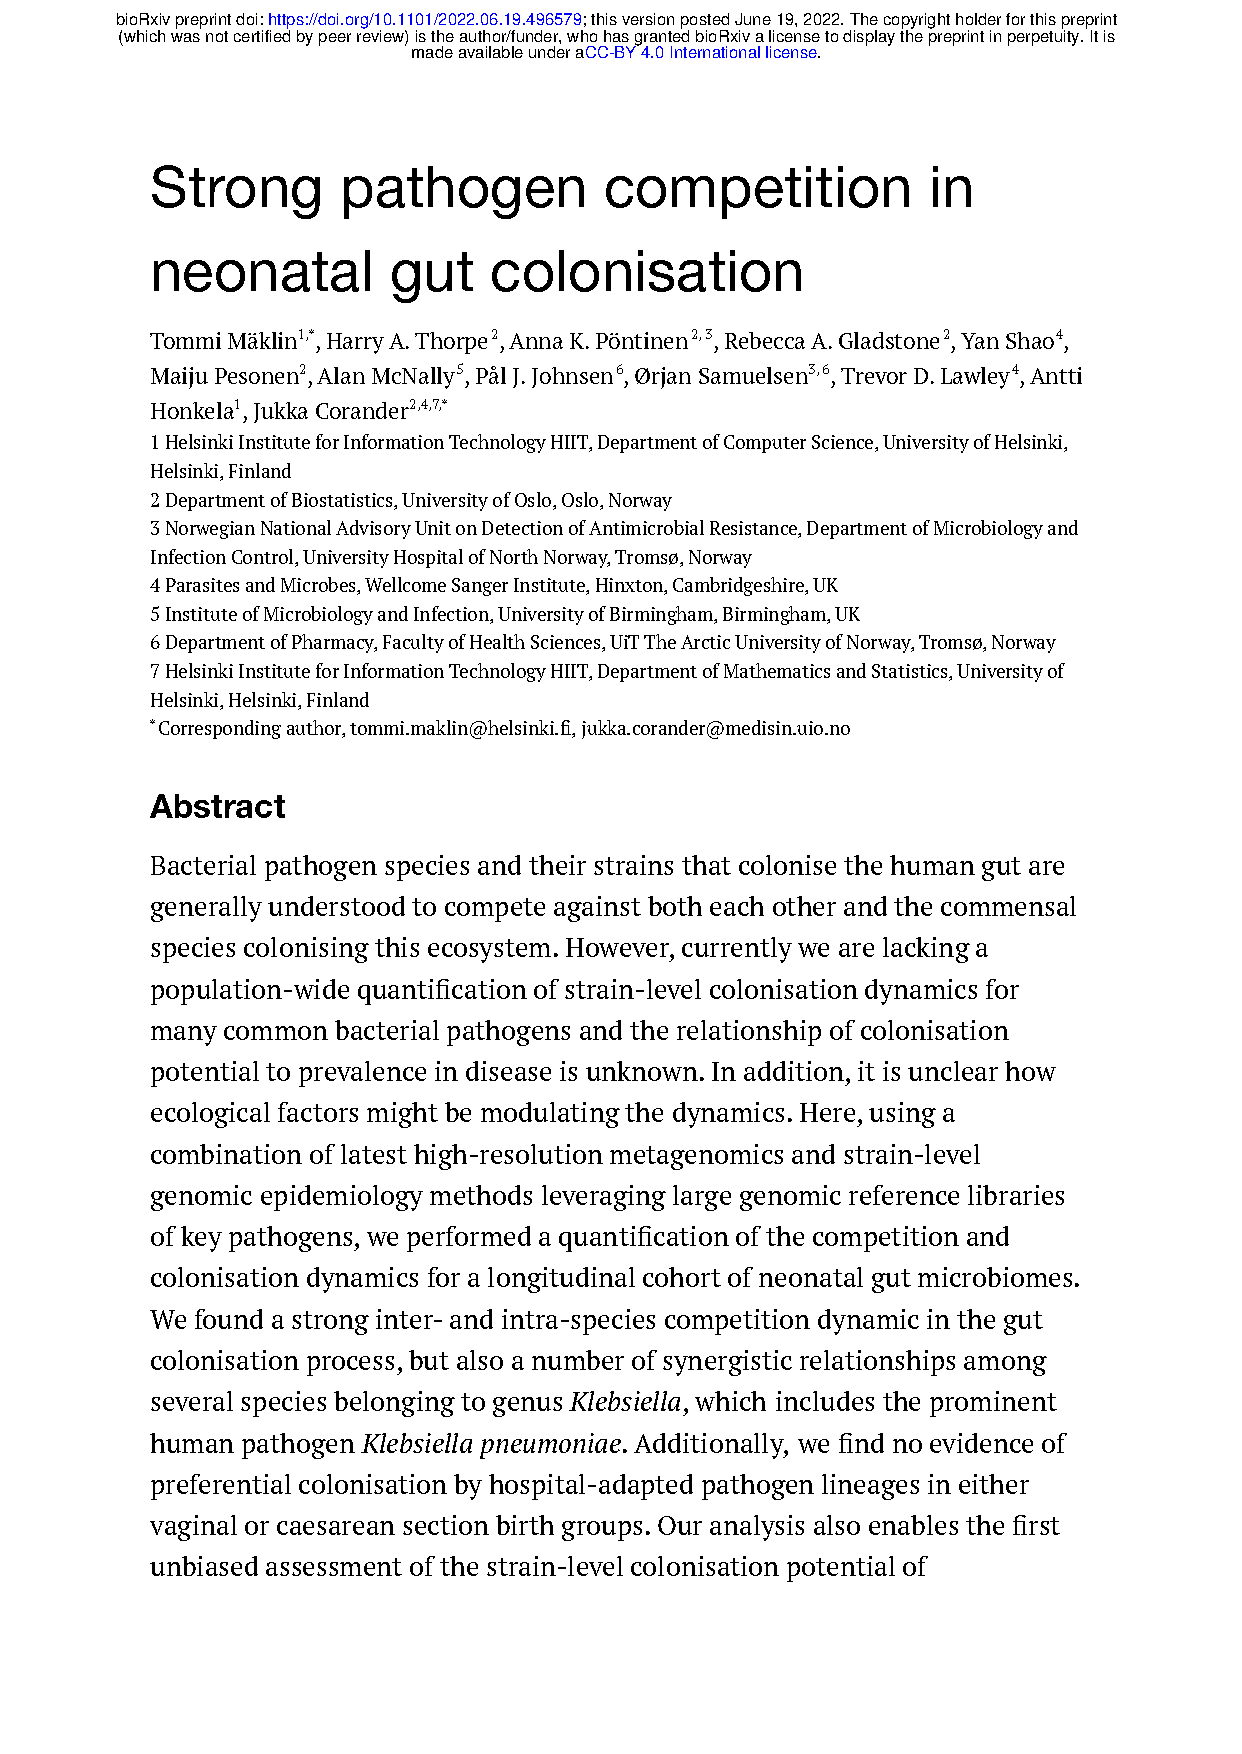
\includepdf[pages=-]{papers/maklin_strong_2022.pdf}



% ******************************************************************************


%% \chapter*{Paper IV}\thispagestyle{empty}
%% \note{I}{-222pt}{\dvWHITE}
%% %\notee{-222pt}{\dvWHITE}

%% \note{II}{-100pt}{\dvWHITE}
%% %\notee{-126.5pt}{\dvWHITE}

%% \note{III}{-5pt}{\dvWHITE}
%% %\notee{-126.5pt}{\dvWHITE}

%% \note{IV}{-5pt}{black}
%% %\notee{-126.5pt}{\dvWHITE}

%% \note{V}{-5pt}{\dvWHITE}
%% %\notee{-126.5pt}{\dvWHITE}

%% \note{VI}{-5pt}{\dvWHITE}
%% %\notee{-126.5pt}{\dvWHITE}

%% \vspace{80pt}
%% % Here are the names of the authors
%% John Doe, Jane Doe, and John Smith

%% \vspace{10pt}
%% % Title of the 4th paper
%% \noindent\textbf{This is the title of the 4th paper}

%% \vspace{10pt}
%% % Bibliographical information of the paper, for example, of a journal paper
%% \noindent
%% In \emph{Journal name}, \\Volume xx, 20ZZ, pages XX-YY.

%% \vspace{60pt}
%% % Copyright information, when the authors have the copyright
%% \noindent Copyright \textcopyright\ The Authors.

%% \cleardoublepage
%% % Including the original publication
%% \includepdf[pages=-]{Publication_name_4.pdf}

% ******************************************************************************

\restoregeometry

%\end{document}
